\documentclass[journal]{IEEEtran}
\usepackage[utf8]{inputenc}
\usepackage{amsmath}
\usepackage{amsfonts}
\usepackage{amssymb}
\usepackage{graphicx}
\usepackage[left=2cm,right=2cm,top=2cm,bottom=2cm]{geometry}
\usepackage[export]{adjustbox}
\usepackage{subfigure,color,amsmath,amssymb,amsfonts}
\usepackage{url,graphicx,subfigure}

% Some handy Latin commands
\newcommand{\etal}{\textit{et al}.}
\newcommand{\ie}{\textit{i}.\textit{e}.,}
\newcommand{\eg}{\textit{e}.\textit{g}.}

\begin{document}
\title{Modeling a MIMO-OFDM Wireless System}
\author{Alon S. Levin\thanks{The Cooper Union, Department of Electrical Engineering}\\Wireless Communications\\ECE-408 --- Spring 2020}
\maketitle

\begin{abstract}

\end{abstract}

\begin{IEEEkeywords}
MIMO, OFDM, pre-coding, zero-forcing, MMSE, IEEE802.11a
\end{IEEEkeywords}

%%%%%%%%%%%%%%%%%%% Introductions %%%%%%%%%%%%%%%%%%
\section{Introduction}\label{sec:intro}

\section{MIMO} \label{sec:MIMO}

\begin{figure}[!htbp]
    \centering
    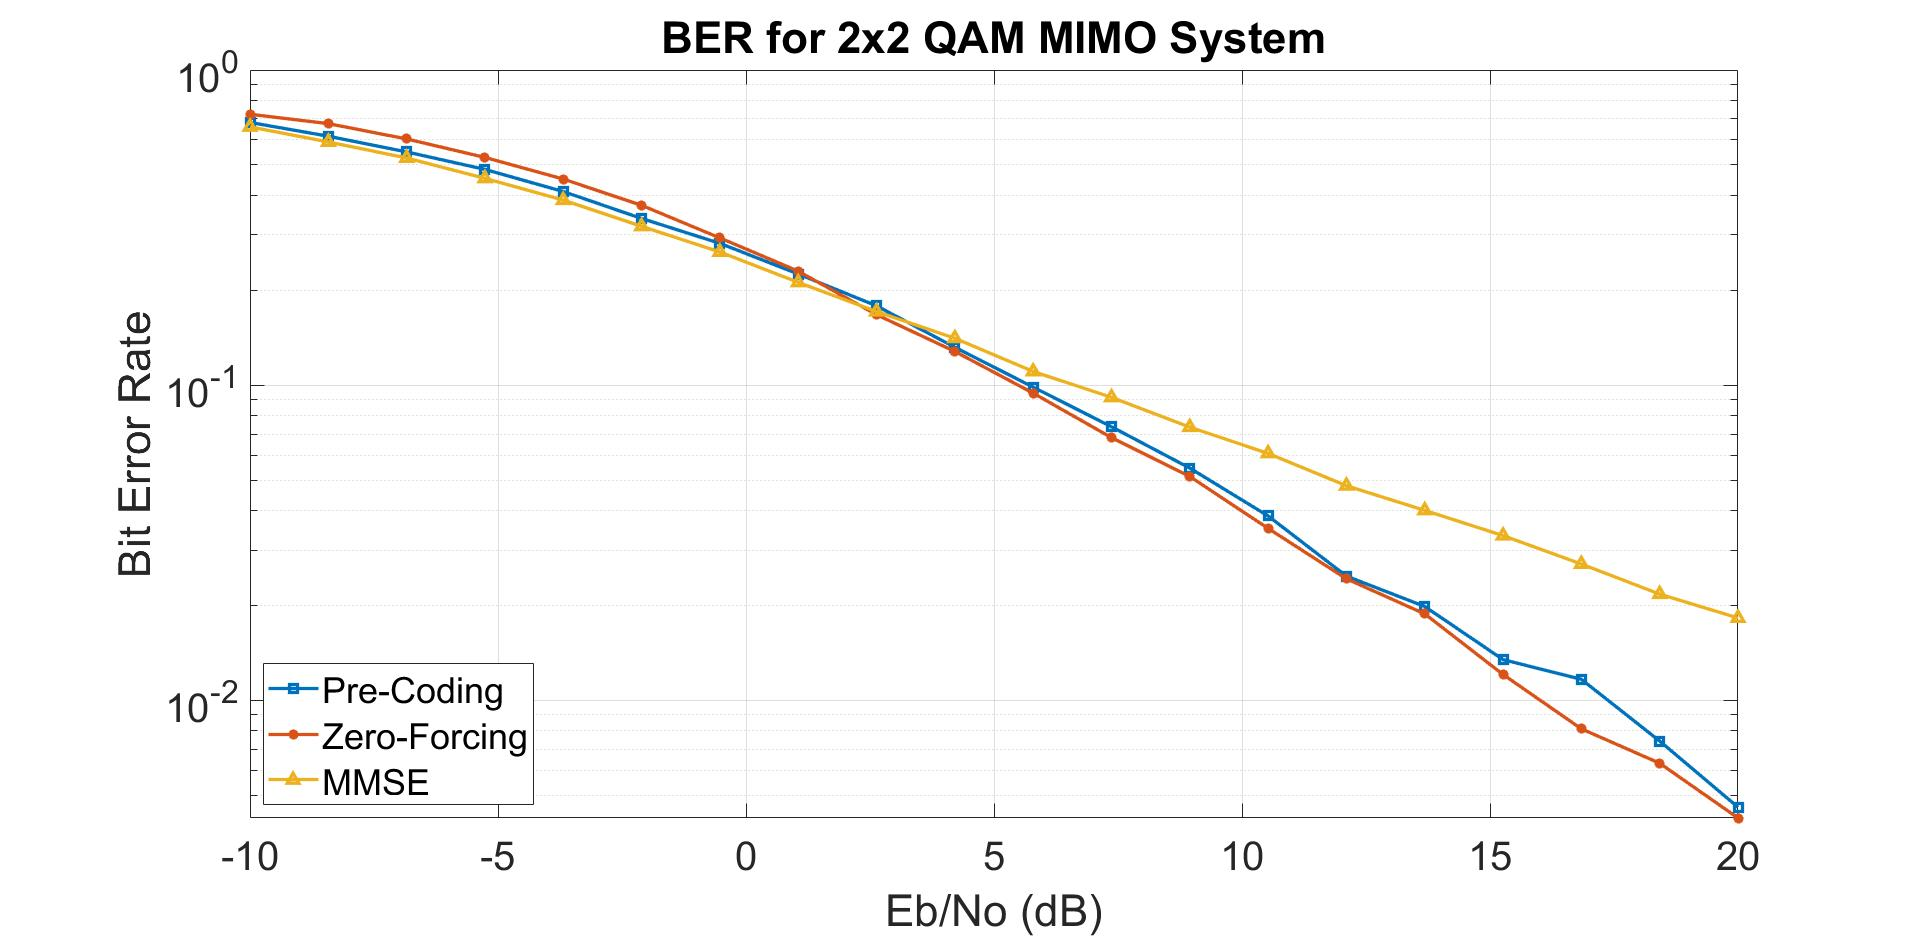
\includegraphics[width = 0.45\textwidth]{MIMO.jpg}
    \caption{BER plot for a $2\times2$ QAM MIMO system using different MIMO algorithms.}
    \label{fig:mimo_res}
\end{figure}

\section{OFDM} \label{sec:OFDM}

\begin{figure}[!htbp]
    \centering
    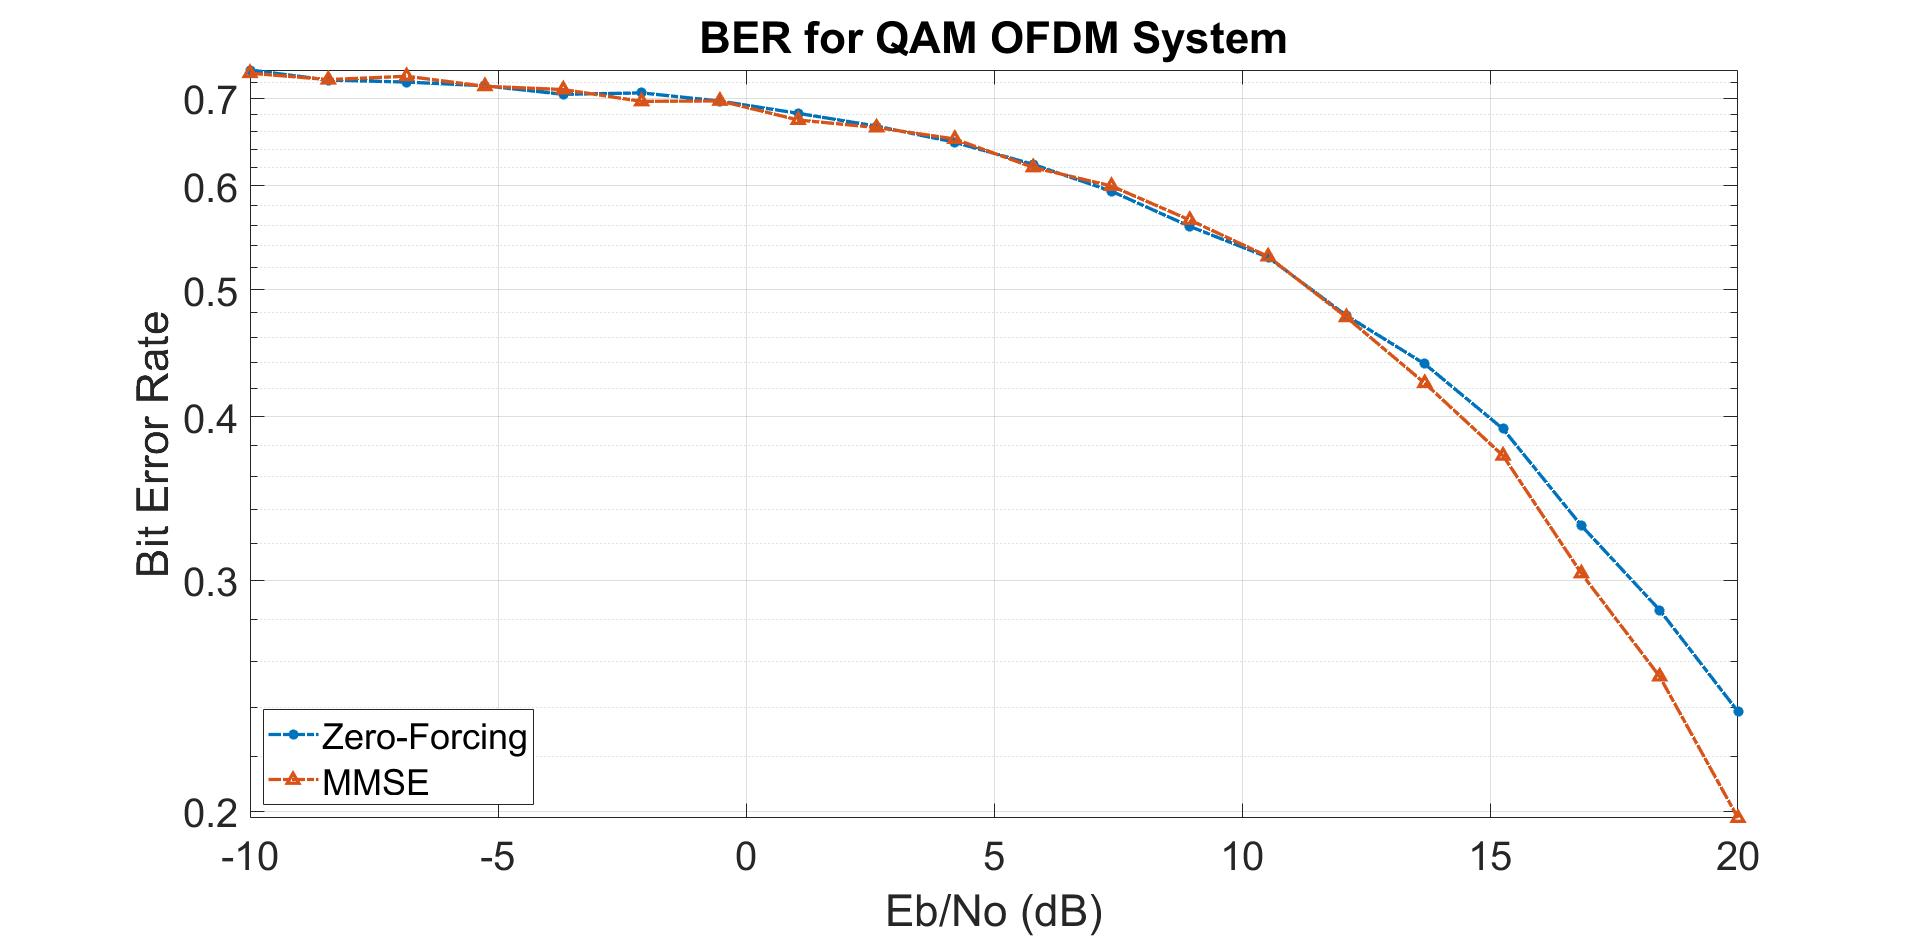
\includegraphics[width = 0.45\textwidth]{OFDM.jpg}
    \caption{BER plot for a QAM OFDM system using different OFDM algorithms.}
    \label{fig:ofdm_res}
\end{figure}

\section{MIMO-OFDM} \label{sec:MIMO-OFDM}

\begin{figure}[!htbp]
    \centering
    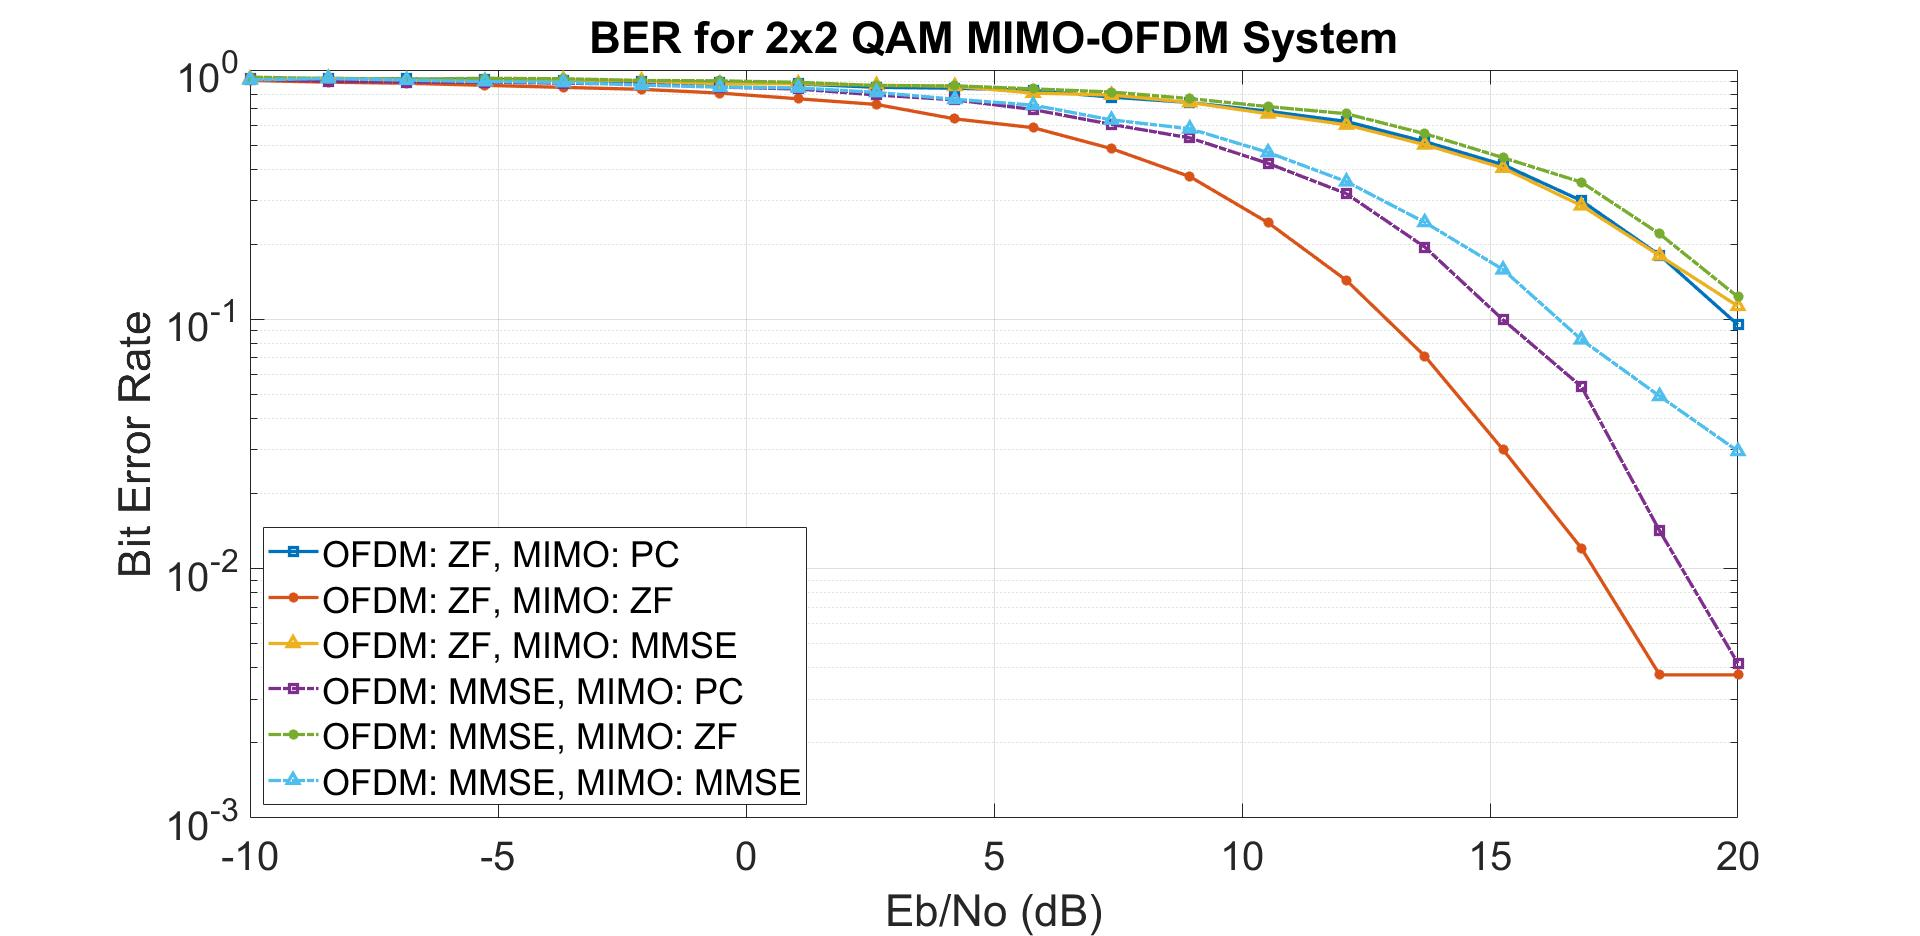
\includegraphics[width = 0.45\textwidth]{MIMOOFDM.jpg}
    \caption{BER plot for a $2\times2$ QAM hybrid MIMO-OFDM system using all combinations of the previous MIMO and OFDM algorithms.}
    \label{fig:mimoofdm_res}
\end{figure}

\section{Conclusion} \label{sec:conc}

%%%%%%%%%%%%%%%%%%% Bibliography %%%%%%%%%%%%%%%%%%%
\bibliographystyle{unsrt}
%% To reload citations:
%% F6 --> F11 --> F6 --> F6 --> F7
\bibliography{Bibliography} %filename (no .bib)

\end{document}